\documentclass{beamer}

\title[GridCertLib]{%
  \emph{GridCertLib} 
  \\
  Shibboleth authentication for X.509 certificates and Grid proxies
}
\author[R.\ Murri]{Riccardo Murri
  \\ \texttt{<riccardo.murri@uzh.ch>}}%
\institute[GC3, University of Zurich]%
{\href{http://www.gc3.uzh.ch/}{Grid Computing Competence Centre}, 
  \\ \href{http://www.uzh.ch/}{University of Zurich}
  \\ \url{http://www.gc3.uzh.ch/}}%
\date{EGI TF 2011}%

\usepackage{ucs}
\usepackage[utf8x]{inputenc}
\usepackage[english]{babel}
\usepackage{array}
\usepackage{color}
\usepackage{fancyvrb}
\usepackage{graphicx}
%\usepackage[spaces,hyphens]{url}
\usepackage{hyperref}
%\usepackage{pslatex}

\newcommand{\cmd}{\begingroup \urlstyle{tt}\Url}  % see url.sty
\newcommand{\file}{\begingroup \urlstyle{tt}\Url}  % see url.sty
\newcommand{\+}{\vspace{1em}}


\usetheme{egi}
\begin{document}

\begin{frame}
\maketitle
\end{frame}



\section[Introduction]{Introduction}

\begin{frame}
  \frametitle{The Problem with Portals}
  \begin{center}
    {\Huge How to get a Grid proxy \\ into the portal host?}
  \end{center}
\end{frame}


% \begin{frame}
%   \frametitle{Portals and MyProxy, today}

%   \begin{enumerate}
%   \item\label{item:proxy} From a command-line UI run
%     \texttt{myproxy-init --voms} \dots
%   \item Log in to portal \dots
%   \item set MyProxy server \dots
%   \item and run jobs.
%   \item When proxy expires, go back to step~\ref{item:proxy}.
%   \end{enumerate}
  
%   \+
%   This is too distracting to most users.

%   \+
%   In addition, resorting to command-line kinda defeats the whole
%   purpose of having a portal\dots
% \end{frame}


\begin{frame}
  \frametitle{What is GridCertLib?}
  
  Java library to create an X.509 certificate and a VOMS proxy upon
  successful login to the portal.

  \+ 
  \emph{For Users:} No interaction with Grid middleware required at all.

  \+
  \emph{For programmers:} assures that, once a user has logged in, valid
  certificate and proxy are available.

  \+
  \emph{Key ingredients:}
  \begin{itemize}
  \item Shibboleth federated authentication
  \item SLCS online CA
  \end{itemize}

\end{frame}


\subsection[AAI Infrastructure]{The SWITCH AAI Infrastructure}

\begin{frame}[label=shib]
  \frametitle{Shibboleth}
  %\framesubtitle{federated authentication mechanism}
    \begin{itemize}
    \item HTTP-based operation
    \item User credentials are authenticated by the
      home organization \emph{Identity Provider} (IdP) server only
      \begin{itemize}
      \item IdP controls what information about the authenticated user
        is sent to the \emph{Service Provider} (SP)
      \item Passwords and other sensitive data are never disclosed to
        Service Providers
      \end{itemize}
    \item \emph{Service Providers} only need to trust the limited number
      of IdPs for authentication purposes.
    \end{itemize}
    
    \+
    \hyperlink{more-shib}{\beamergotobutton{Shibboleth login workflow}}
\end{frame}


\begin{frame}
  \frametitle{The SWITCH AAI Infrastructure}
  {\Large Switzerland-wide federated authentication infrastructure.}
  \begin{itemize}
  \item Based on Shibboleth 2.x
  \item ``Identity Providers'' already operational at every University
    and several other research centres.
  \item One login/password to access a variety of services
    (e.g., e-mail, ... and SLCS!)
  \end{itemize}
\end{frame}


\begin{frame}[label=slcs]
  \frametitle{Short-Lived Credential Service}
  Web service to create an X.509 user certificate,
  valid for 11 days.
  \begin{itemize}
  \item A \emph{new} certificate at each successful invocation
  \item \emph{Same} subject DN every time
  \item Command-line client (Java-based) available in gLite 3.x
  \end{itemize}

  \+ {\em Uses AAI/Shibboleth authentication.}

  \+ SWITCH SLCS CA is already in the IGTF bundle
  \begin{itemize}
  \item SLCS certificates can be used for normal Grid operations
  \end{itemize}

  \+
  {\em Already in use in SMSCG, the Swiss national Grid infrastructure.}

  \+
  \hyperlink{more-slcs}{\beamergotobutton{More on SLCS}}
\end{frame}


\section[Project overview]{GridCertLib operation}

\begin{frame}
  \frametitle{Architecture}
  \begin{center}
    \vskip 4.0em
    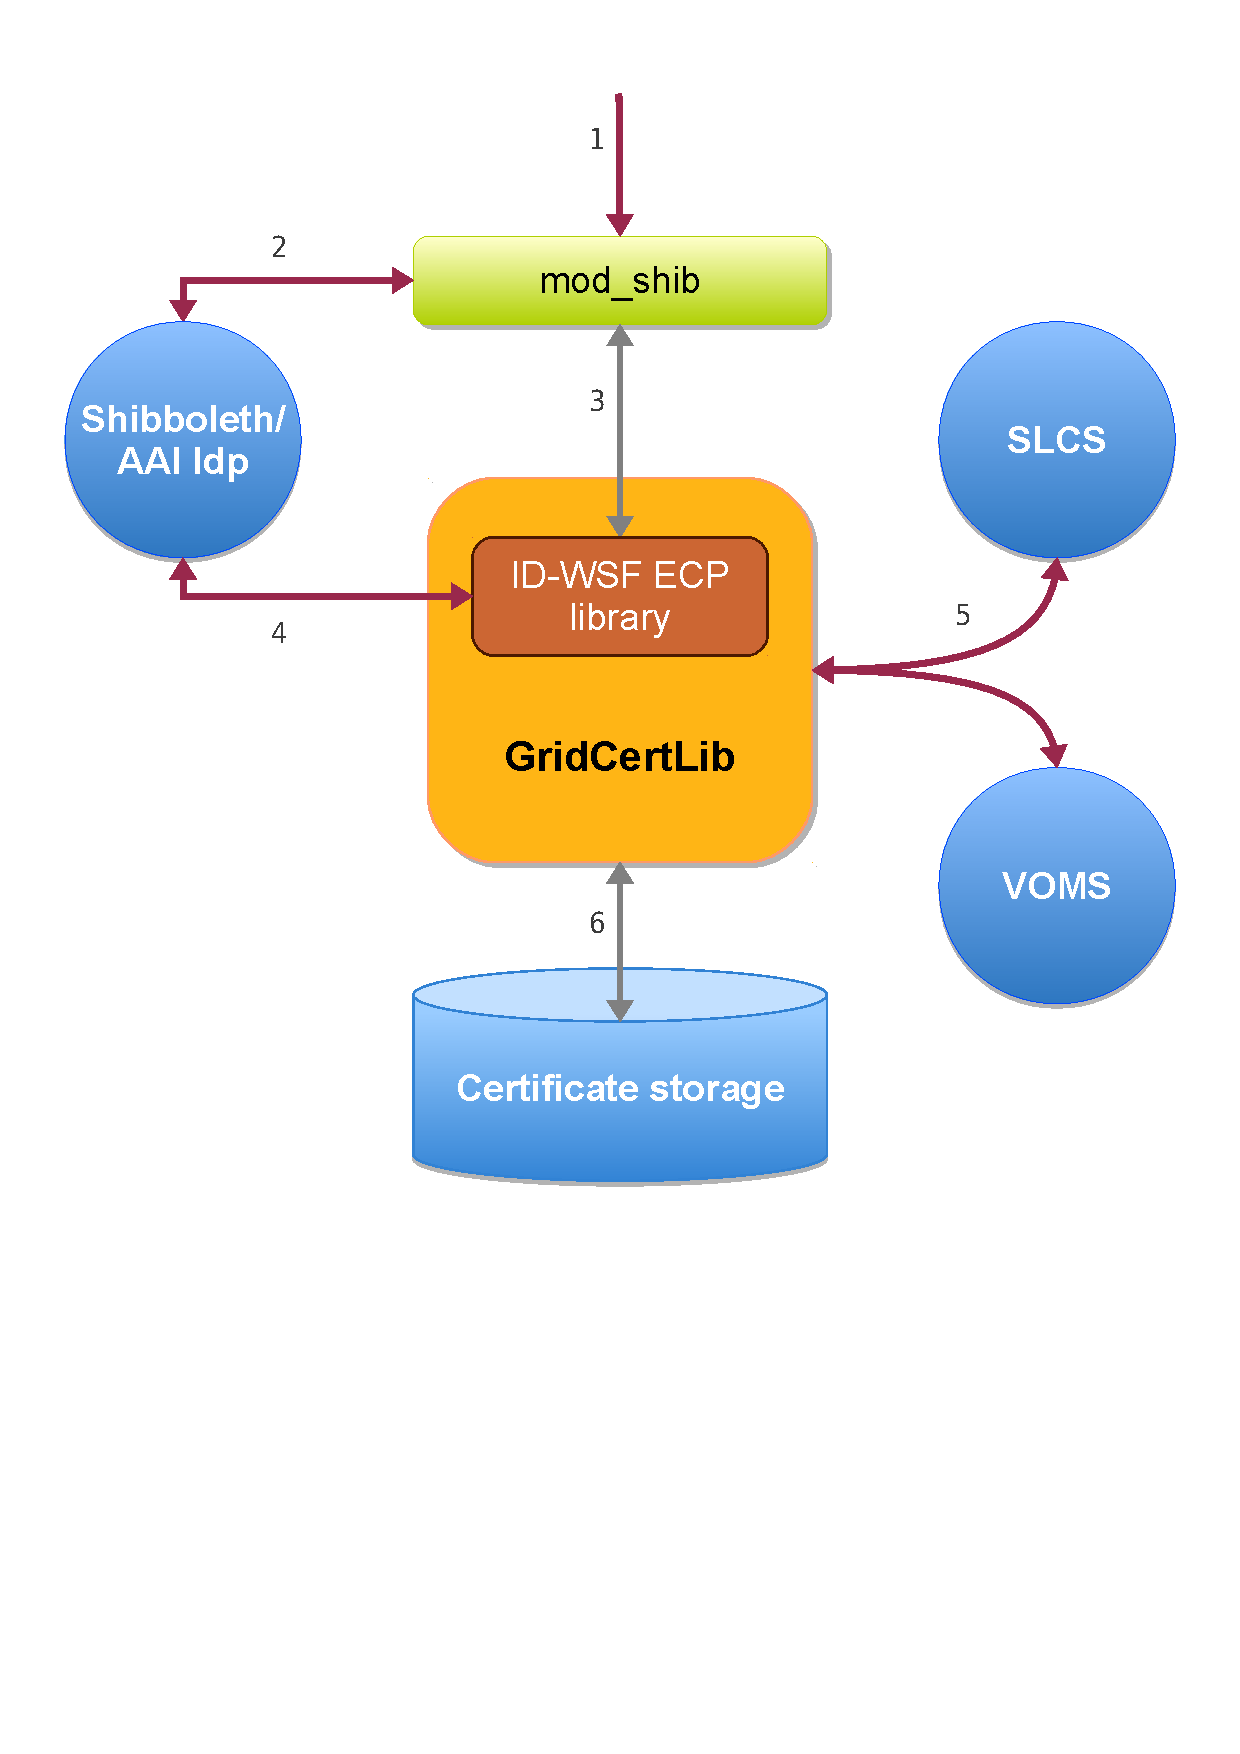
\includegraphics[width=0.66\textwidth,viewport=0 300 600 650]{architecture}
  \end{center}
\end{frame}

\begin{frame}
  \frametitle{GridCertLib operation (1)}
  \begin{center}
    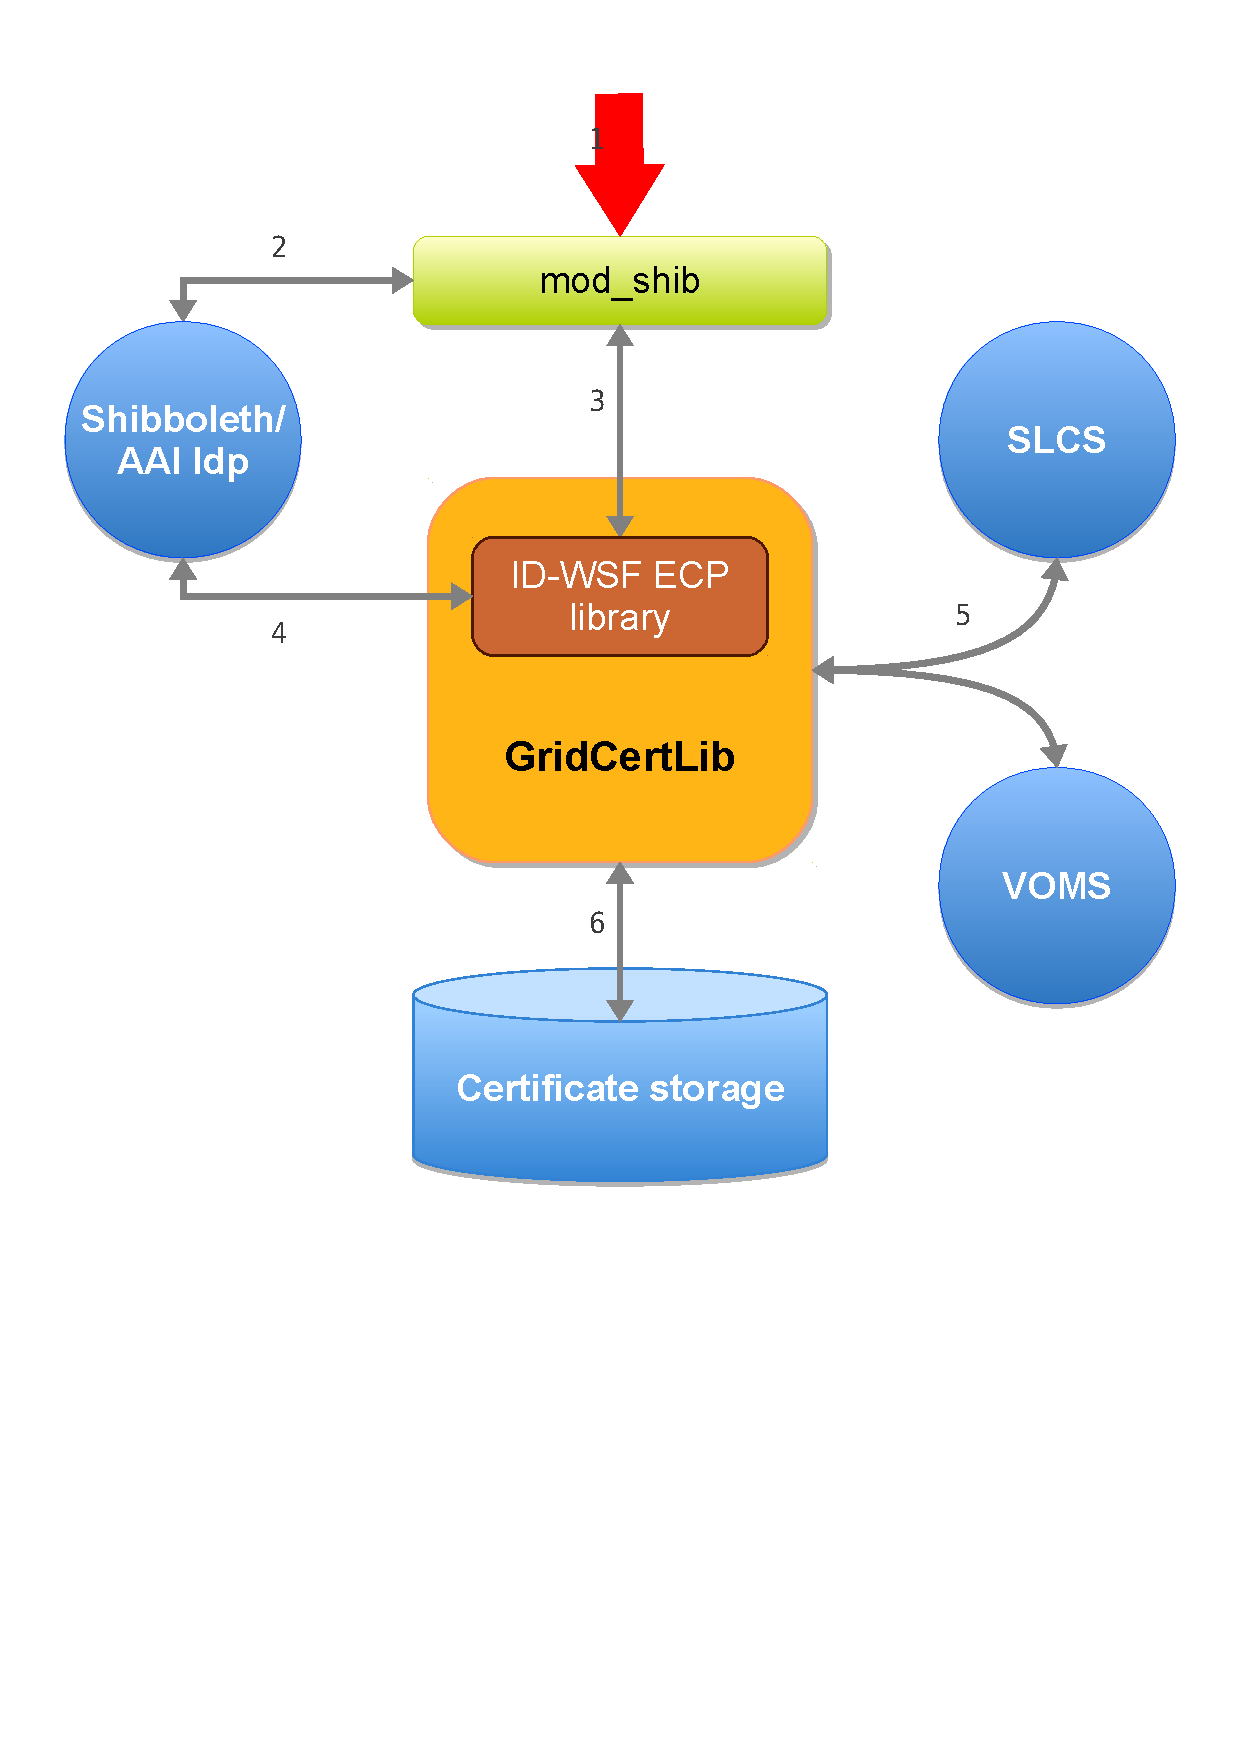
\includegraphics[width=0.5\textwidth,viewport=0 300 600 650]{architecture1}
    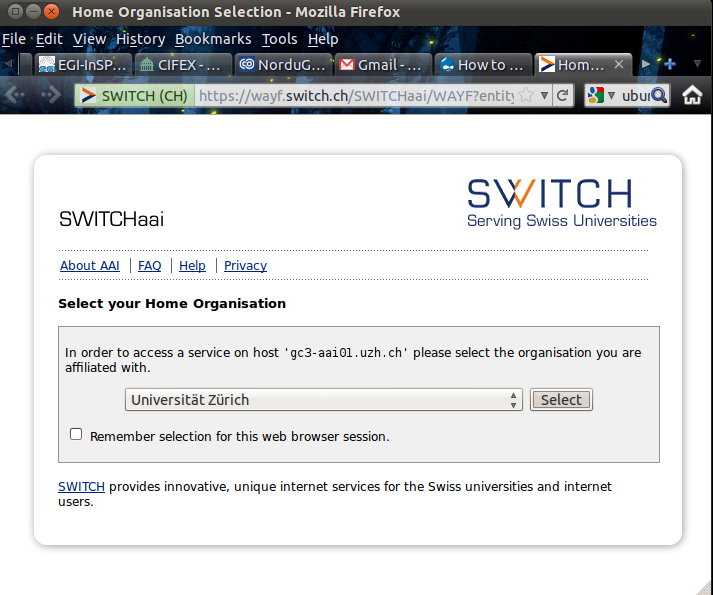
\includegraphics[height=0.50\textheight]{wayf}
  
    \+ Users log in to the web portal using Shibboleth single sign-on.
  \end{center}
\end{frame}


\begin{frame}
  \frametitle{GridCertLib operation (2)}
  \begin{center}
    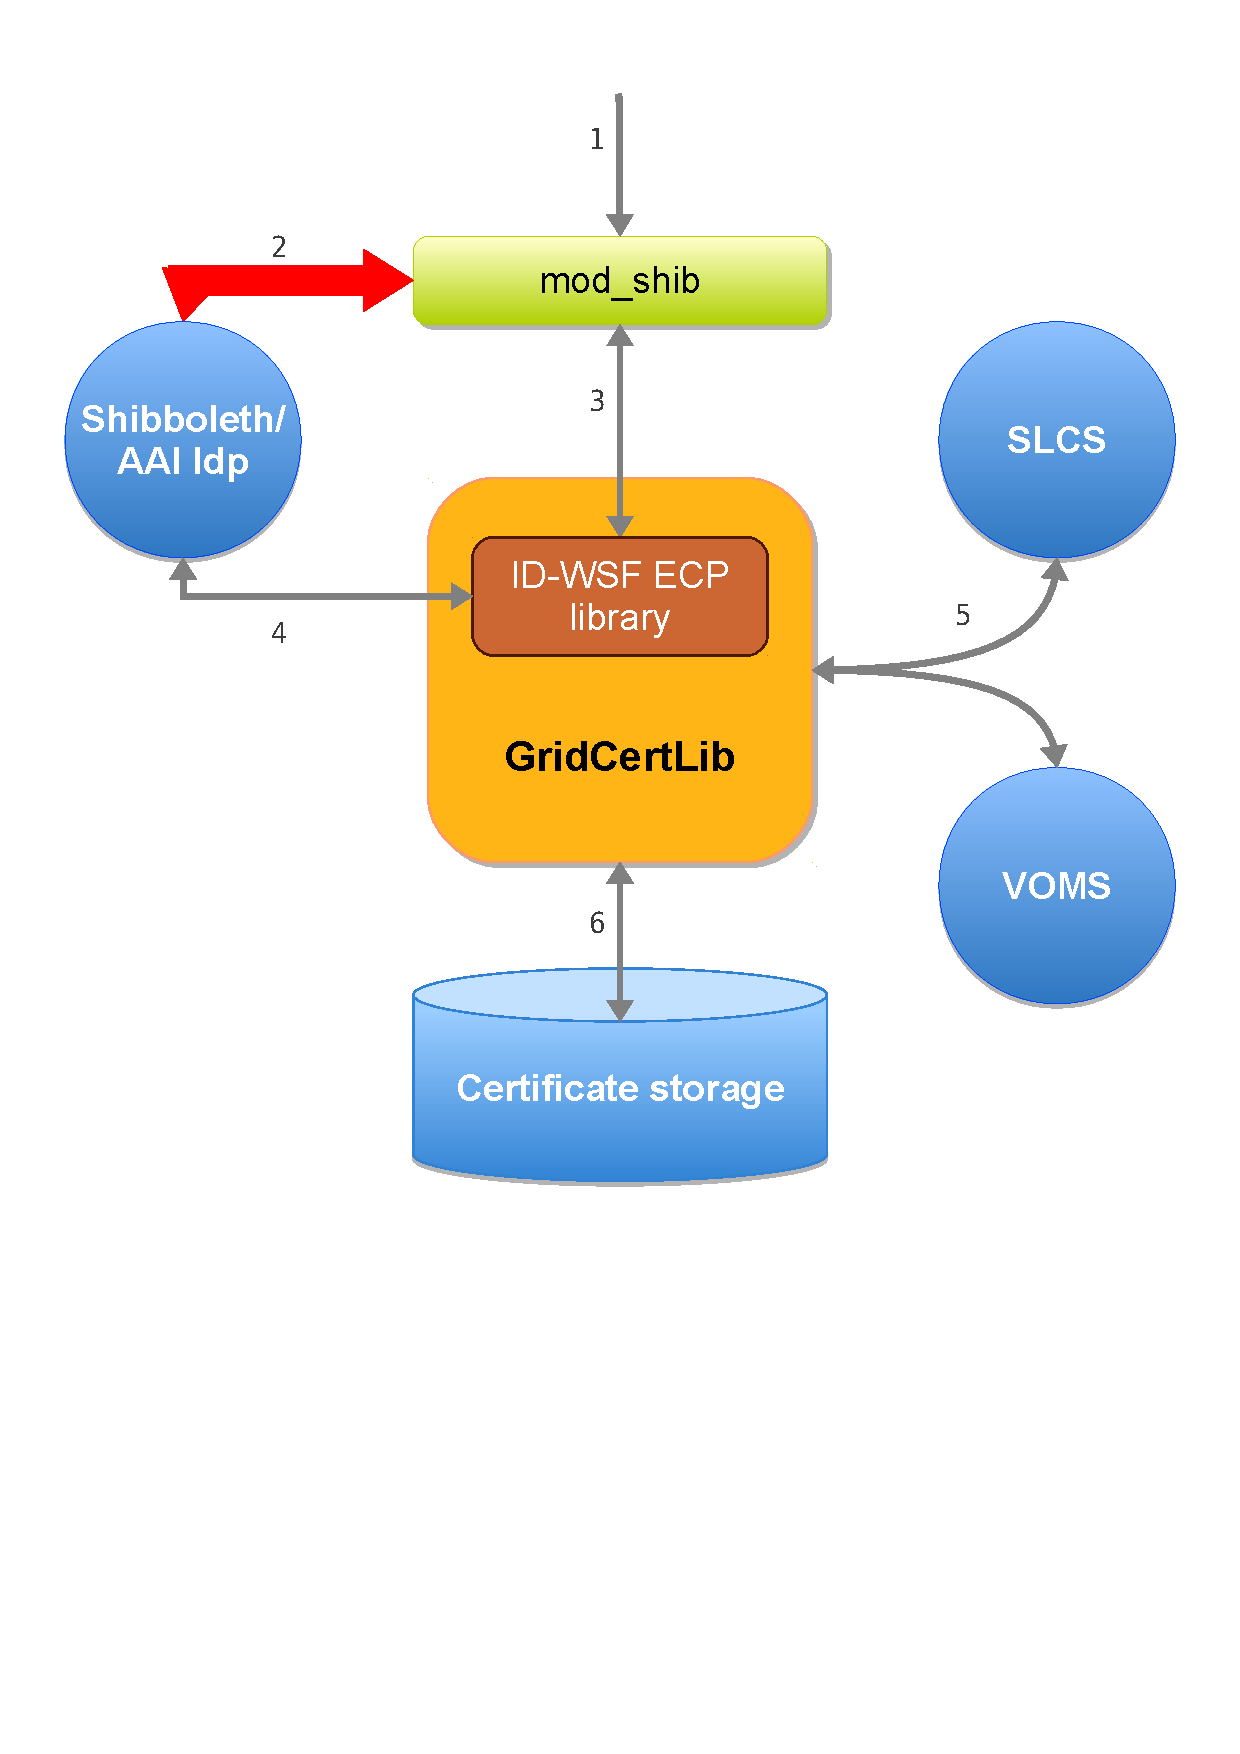
\includegraphics[width=0.5\textwidth,viewport=0 300 600 650]{architecture2}
    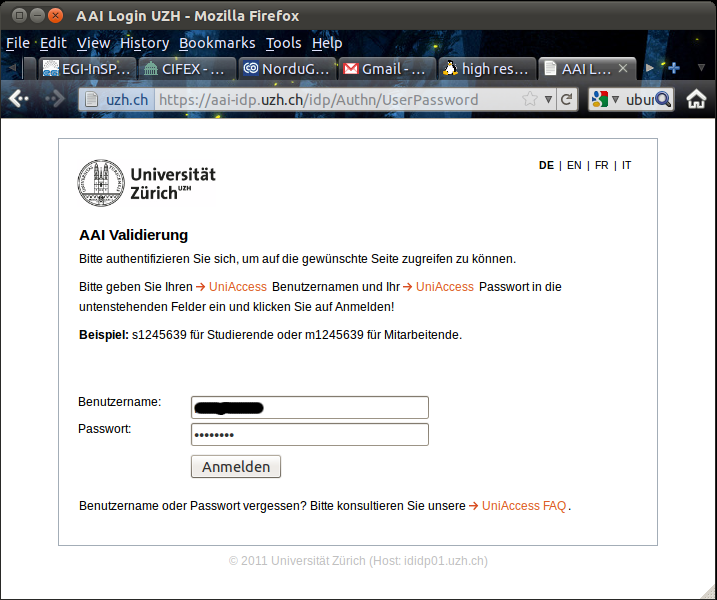
\includegraphics[height=0.50\textheight]{idp}

    \+ Users are authenticated by their home organization ``Identity
    Provider'' (IdP).

    \+ (This is all transparently handled by the Shibboleth software.)
  \end{center}
\end{frame}


\begin{frame}
  \frametitle{GridCertLib operation (3)}
  \begin{columns}
    \begin{column}{0.5\textwidth}
    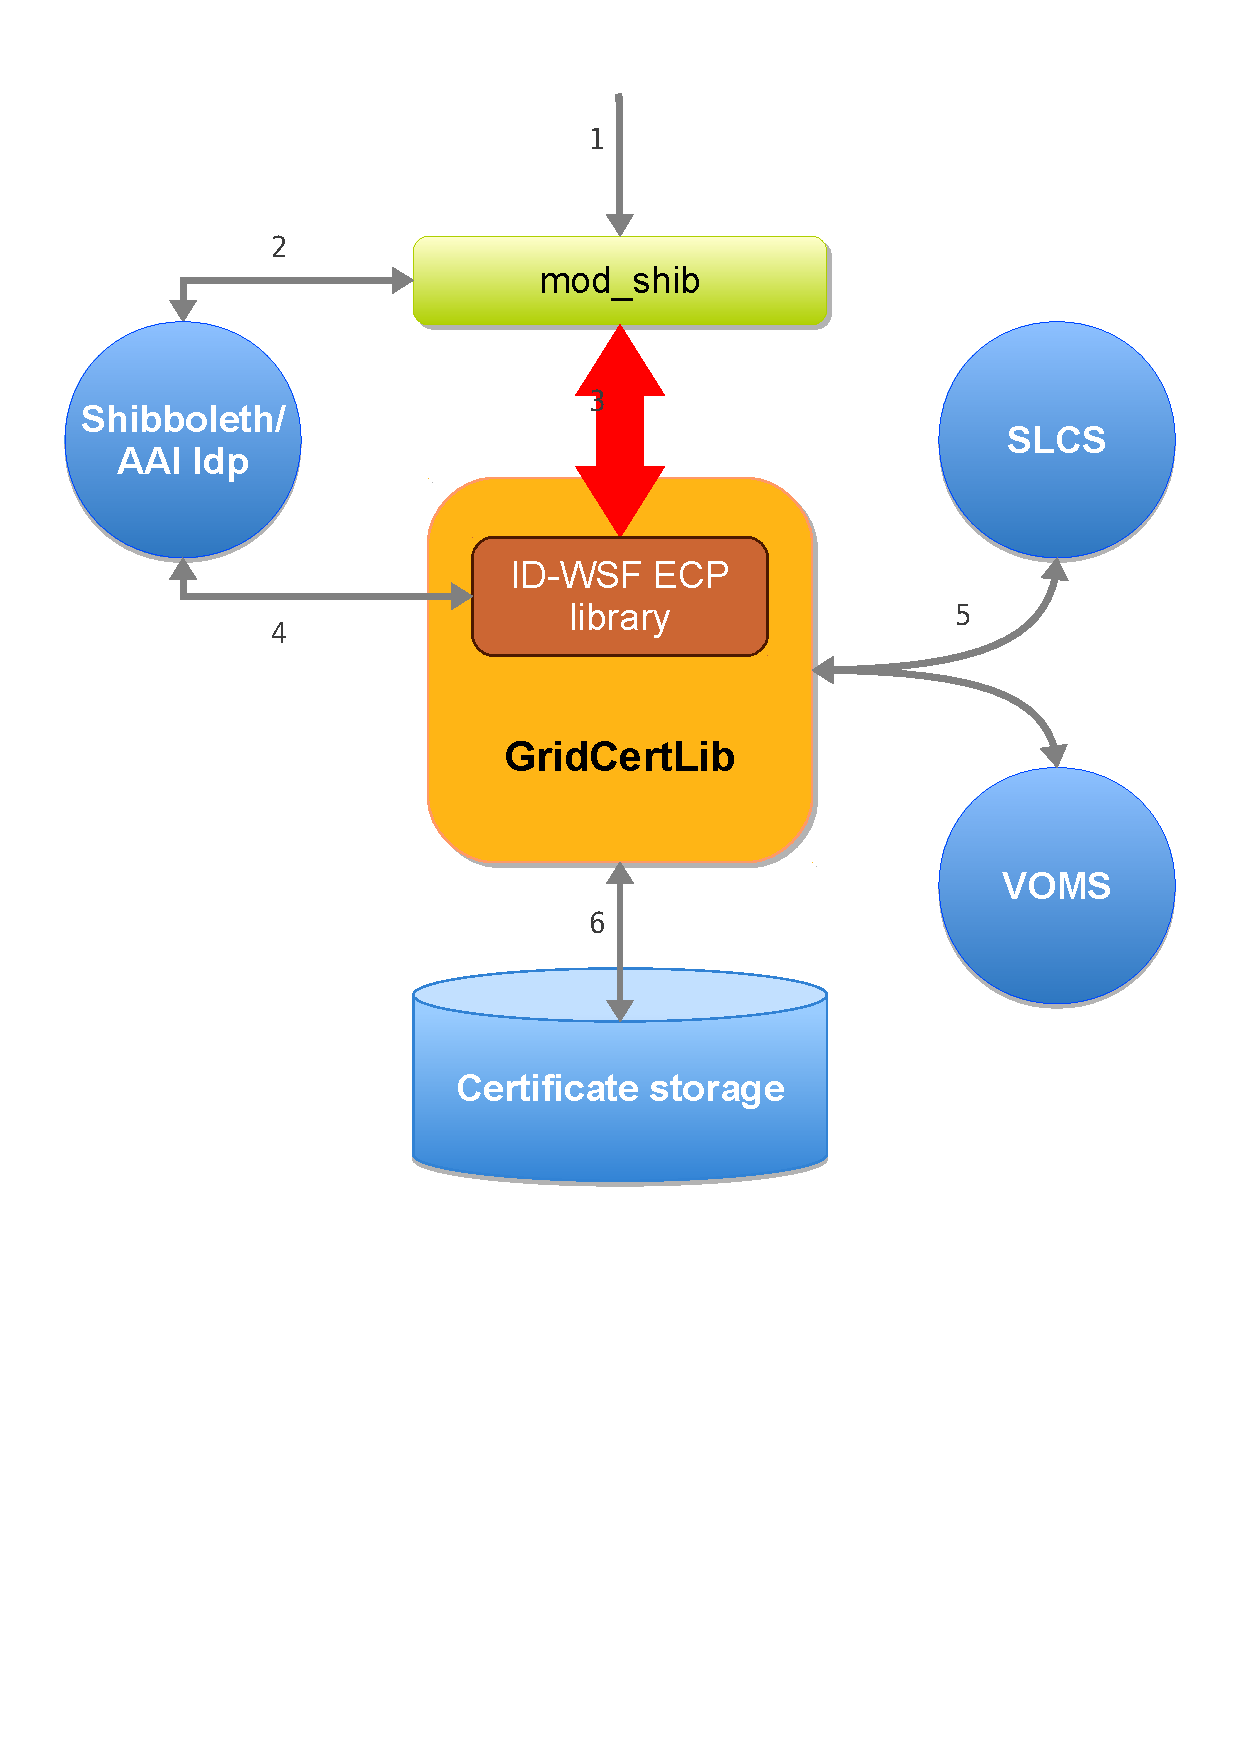
\includegraphics[width=\linewidth,viewport=0 300 600 650]{architecture3}
    \end{column}
    \begin{column}{0.5\textwidth}
      \begin{center}
        The portal calls GridCertLib.
        
        \+ GridCertLib retrieves the SAML2 assertion (Shibboleth login
        data) from Apache's \texttt{mod\_shib}.
      \end{center}
    \end{column}
  \end{columns}
\end{frame}


\begin{frame}
  \frametitle{GridCertLib operation (4)}
  \begin{columns}
    \begin{column}{0.5\textwidth}
    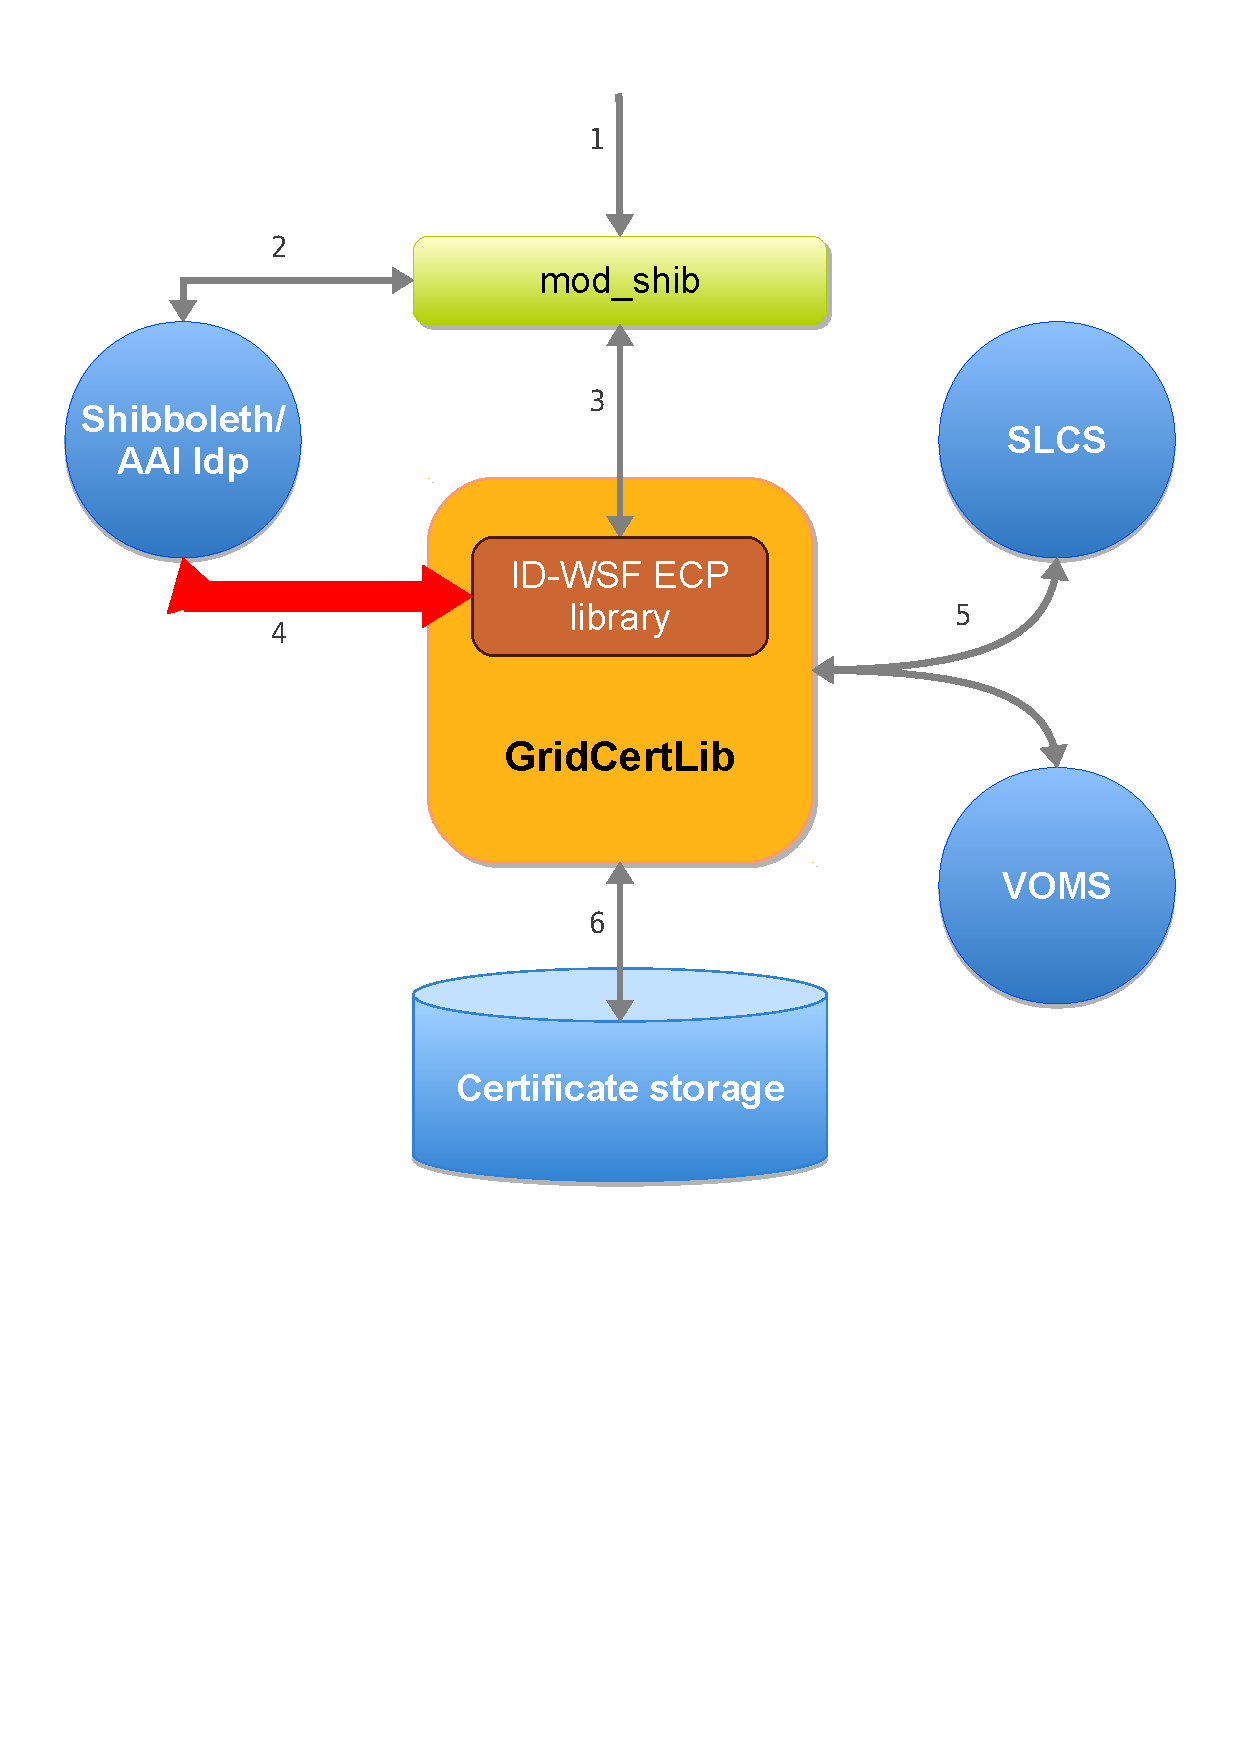
\includegraphics[width=\linewidth,viewport=0 300 600 650]{architecture4}
    \end{column}
    \begin{column}{0.5\textwidth}
      \begin{center}
        GridCertLib generates an X.509 certificate, signs it using
        SLCS, and then generates a VOMS proxy.
      \end{center}
    \end{column}
  \end{columns}
\end{frame}


\begin{frame}
  \frametitle{Techinical issues (1)}
  
  {\bf Obtaining a user certificate requires delegation of the Shibboleth
  credentials to the SLCS login service.}
  \begin{itemize}
  \item SLCS web service requires Shibboleth authentication...
  \item ...but AuthN data is only valid towards SP!
  \end{itemize}

  \+ 
  \emph{Delegation issue}
  \begin{itemize}
  \item Shibboleth 2.1.x supports \emph{delegation} of credentials
  \item but deployed IdP's not (yet) up to that version
  \end{itemize}

  \+
  \emph{Solution}
  \begin{itemize}
  \item use pre-production Shibboleth 2.2 IdP \emph{with delegation extension} (at SWITCH)
  \item register/manage portal user accounts there
  \item will merge with the production infrastructure eventually
  \end{itemize}
\end{frame}


\begin{frame}
  \frametitle{GridCertLib operations (5)}
  \emph{Generate X.509 certificate:}
  \begin{columns}
    \begin{column}{0.4\textwidth}
      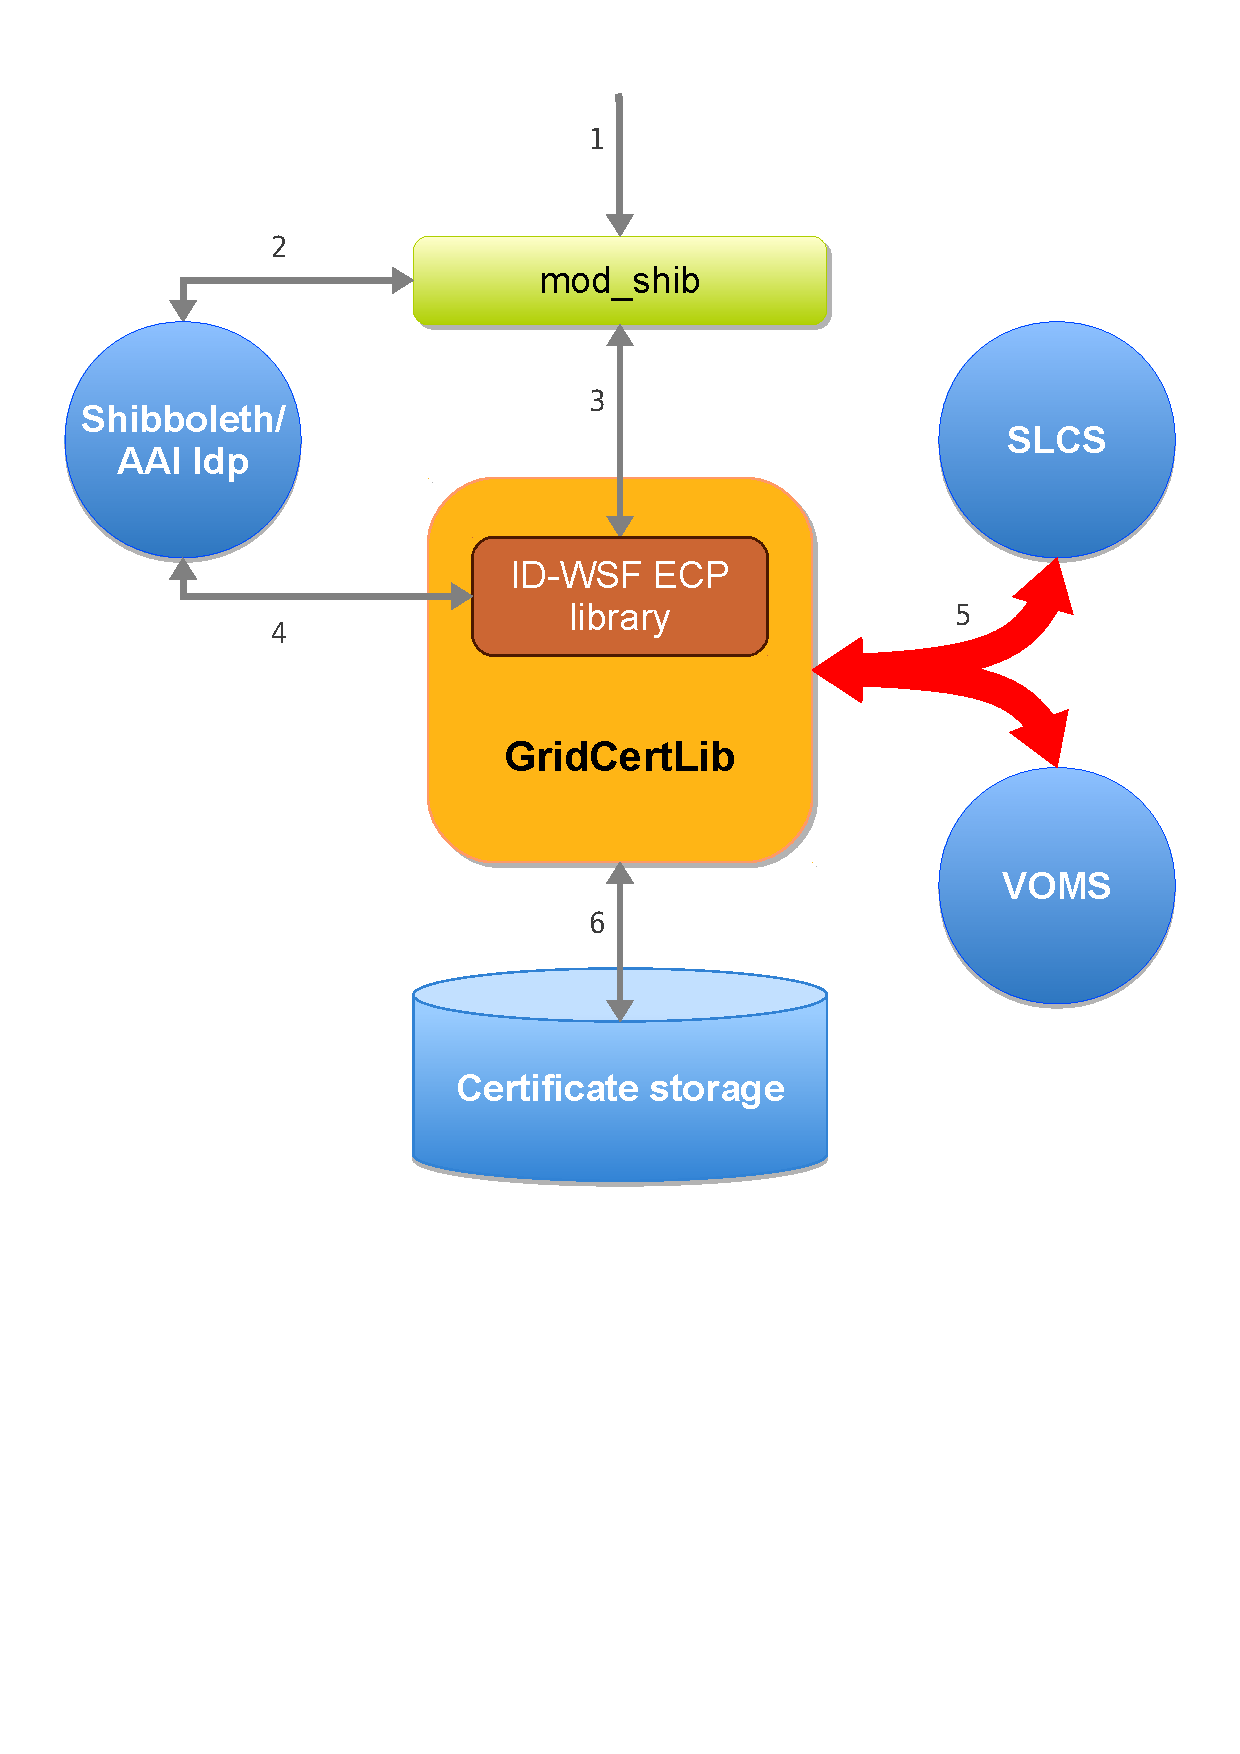
\includegraphics[width=\linewidth,viewport=0 300 600 650]{architecture5}
    \end{column}
    \begin{column}{0.6\textwidth}
      \begin{enumerate}
      \item Login to SLCS endpoint
      \item SLCS server verifies AuthN data with IdP
      \item SLCS replies with a ``session'' token and information
        to generate a CSR
      \item Generate a private key and a CSR
      \item Submit CSR to SLCS endpoint
      \item Get back \emph{signed certificate} in response
      \end{enumerate}
    \end{column}
  \end{columns}

  \emph{Then, generate proxy and contact VOMS server.}
\end{frame}


\begin{frame}
  \frametitle{GridCertLib operations (6)}
  \begin{columns}
    \begin{column}{0.45\textwidth}
      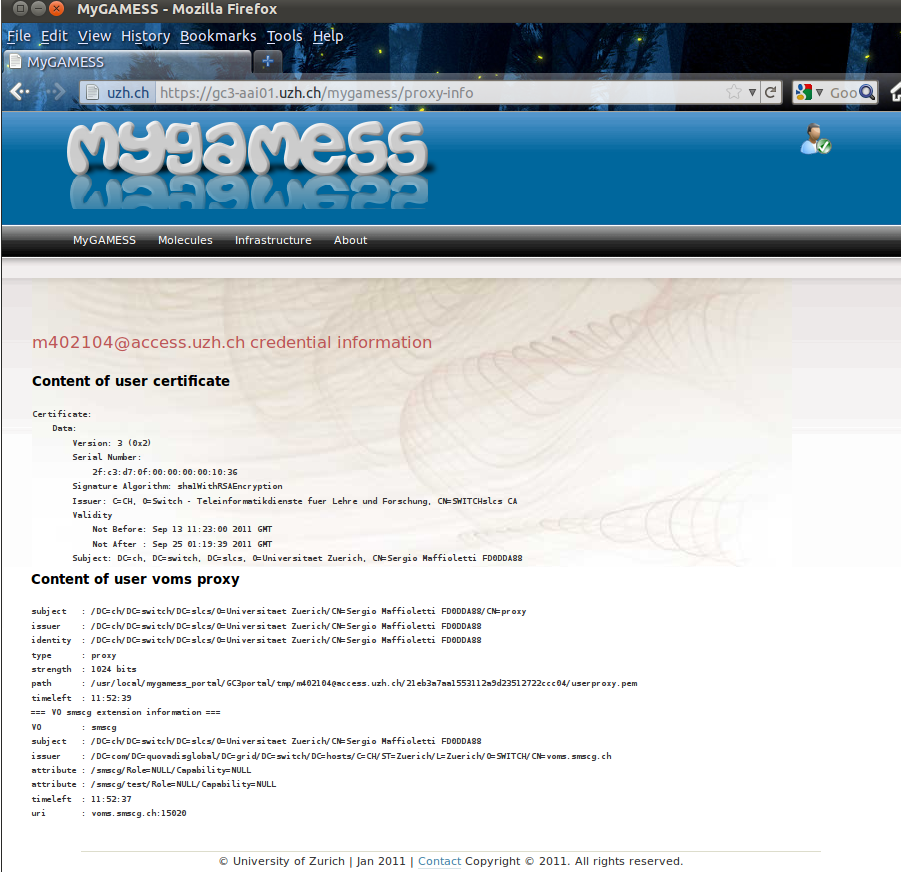
\includegraphics[width=\linewidth]{mygamess}
    \end{column}
    \begin{column}{0.55\textwidth}
      \begin{center}
        Store certificate and proxy on the disk, ready for use.
        \\
        {\footnotesize (Encrypted with a random password, which is
          returned by the GridCertLib API.)}
      
        \+ {Users only interact via WWW, and
          passwords are sent to the IdP only (and only once per
          login!)}
      \end{center}
    \end{column}
  \end{columns}
\end{frame}


\section[Implementation]{Success stories}

\begin{frame}[label=pgrade]
  \frametitle{P-GRADE integration}

  Two main action items:
  \begin{itemize}
  \item Enable Shibboleth login at the GridSphere level
    \begin{itemize}
    \item Initially done by the Australian MAMS project
    \item Requires some lengthy procedure to make login data
      compatible with the DB storage
    \end{itemize}
  \item Insert calls to GridCertLib into the login code
    \begin{itemize}
    \item Java code calling Java code, no big issue
    \end{itemize}
  \end{itemize}

  \hyperlink{more-pgrade}{\beamergotobutton{More on P-GRADE integration}}
\end{frame}


\begin{frame}[fragile]
  \frametitle{Django integration}

  \emph{Issue:} How to bridge Python with Java?
  \begin{itemize}
  \item Run \emph{GridCertLib} servlets in parallel with Django.
  \item Use HTTP redirects to pass information back and forth.
  \end{itemize}

  \+
  Use Python decorators to mark view functions that require a
  certificate and/or Grid proxy.
\begin{verbatim}
  @proxy_required
  def submit_job(req):
    # do Grid work
    return HttpResponse(...)
\end{verbatim}

\end{frame}


\section{Conclusion}
\label{sec:conclusion}

\begin{frame}[label=summary]
  \frametitle{Summary}
  
  Java library to create an X.509 certificate and a VOMS proxy upon
  successful login to the portal.
  \begin{itemize}
  \item No user interaction with Grid middleware required at all.
  \item Once a user has logged in, valid certificate and proxy are
    available.
  \end{itemize}

  \+
  Already integrated with P-GRADE and Django
  \begin{itemize}
  \item Example servlets with commented code provided for integration
    in other portals.
  \end{itemize}

  \+
  \emph{Key ingredients:}
  \begin{itemize}
  \item Shibboleth federated authentication
  \item SLCS online CA
  \end{itemize}
\end{frame}


\begin{frame}
  \frametitle{Any questions?}
  \begin{center}\Large
    website: \url{http://gridcertlib.googlecode.com/}

    \+
    {e-mail: \\ \texttt{riccardo.murri@uzh.ch}, \texttt{peter.kunszt@systemsx.ch}}

    \+
    \textbf{Credits} \\
    Peter Kunszt~(SystemsX.ch),
    Sergio~Maffioletti~(GC3/UZH),
    Valery~Tschopp~(SWITCH)
  \end{center}
\end{frame}


\againframe{summary}


\section{Appendices}


\subsection{Shibboleth login workflow}

\begin{frame}[label=more-shib]
  \frametitle{Shibboleth login workflow / 1
    \hfill%
    {\tiny (Images courtesy of 
      \href{http://www.switch.ch/aai/demo/2/medium.html}{SWITCH})}
  }
  \begin{center}
    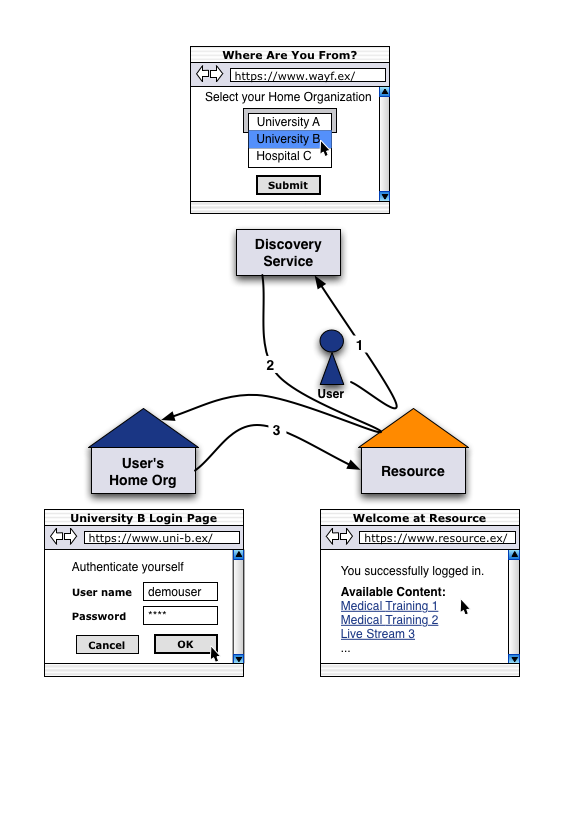
\includegraphics[height=0.66\textheight]{simple_complete}
  \end{center}
  \begin{enumerate}
  \item[1] User first connects to portal web server (SP) and is
    redirected to the ``Where Are You From?'' page (WAYF)
  \end{enumerate}
\end{frame}


\begin{frame}
  \frametitle{Shibboleth login workflow / 2
    \hfill%
    {\tiny (Images courtesy of 
      \href{http://www.switch.ch/aai/demo/2/medium.html}{SWITCH})}
  }
  \begin{center}
    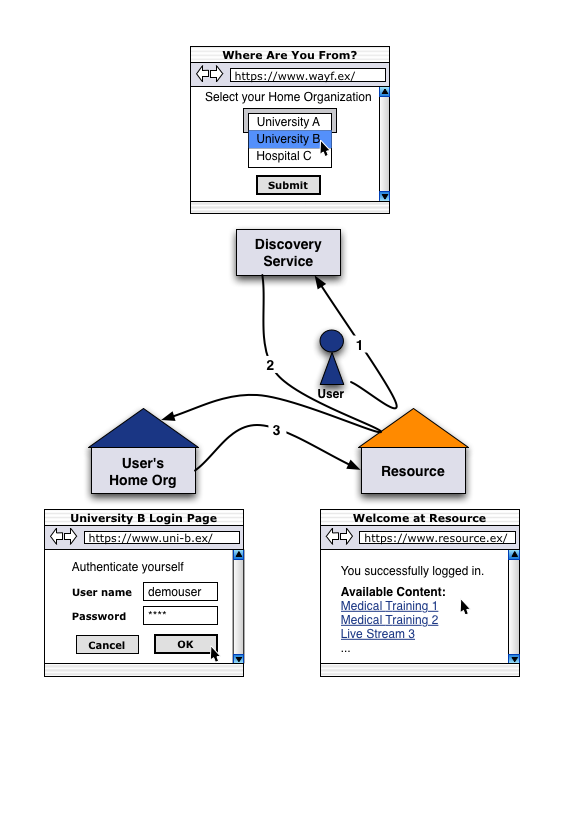
\includegraphics[height=0.66\textheight]{simple_complete}
  \end{center}
  \begin{enumerate}
  \item[2] User chooses Home Organisation and is redirected to the IdP
    AuthN page
  \end{enumerate}
\end{frame}


\begin{frame}
  \frametitle{Shibboleth login workflow / 3
    \hfill%
    {\tiny (Images courtesy of 
      \href{http://www.switch.ch/aai/demo/2/medium.html}{SWITCH})}
  }
  \begin{center}
    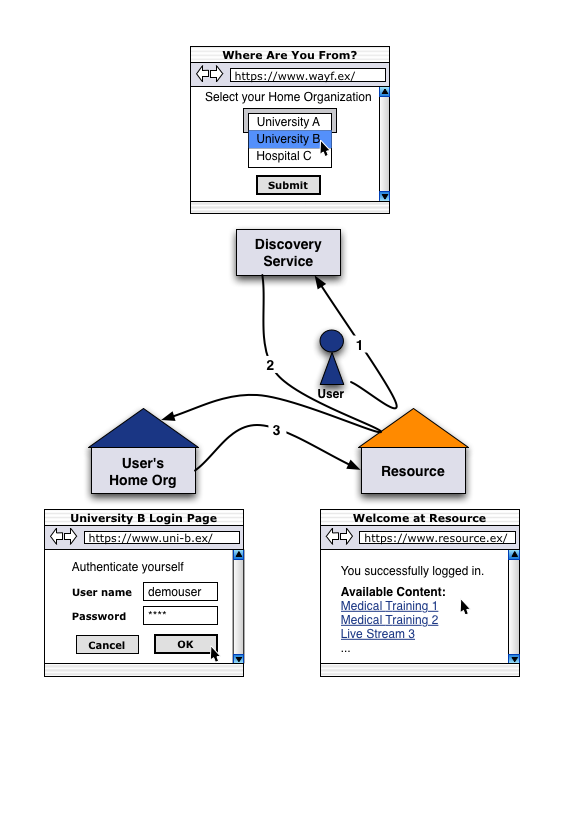
\includegraphics[height=0.66\textheight]{simple_complete}
  \end{center}
  \begin{enumerate}
  \item[3] User posts username/password to IdP and is redirected to
    original page on SP
    \begin{itemize}
    \item Detailed workflow much more convoluted; see extra slides at end.
    \end{itemize}
  \end{enumerate}

  \+
  \hyperlink{shib}{\beamergotobutton{Back to Shibboleth Intro}}
\end{frame}


\subsection{SLCS workflow}

\begin{frame}[label=more-slcs]
  \frametitle{SLCS operations workflow}
  \begin{enumerate}
  \item Login to SLCS endpoint
    \begin{itemize}
    \item HTTP request, using SAML assertion as AuthN data
    \end{itemize}
  \item SLCS server verifies AuthN data with IdP
    \begin{itemize}
    \item Need delegation functionality (Shibboleth 2.1)
    \end{itemize}
  \item\label{item:2} SLCS replies with a ``session'' token and information
    to generate a CSR
  \item Generate a private key and a CSR
    \begin{itemize}
    \item Private key protected by random password known only to the portal
    \end{itemize}
  \item Submit CSR to SLCS endpoint
    \begin{itemize}
    \item Use ``session'' token from step~\ref{item:2}
    \end{itemize}
  \item Get back signed certificate in response
  \end{enumerate}

  \+
  \hyperlink{slcs}{\beamergotobutton{Back to SLCS Intro}}
\end{frame}


\begin{frame}
  \frametitle{More technical issues}
  
  \textbf{Shibboleth authentication data has a limited time validity}
  \begin{itemize}
  \item By the time GridCertLib is called, it might have expired.
  \end{itemize}

  \+
  \textbf{Solution}
  \begin{itemize}
  \item Use a ``RenewAssertion'' servlet \texttt{http://example.com/RenewAssertion?url=...}
  \item Forces Shibboleth logout
  \item Redirects to whatever URL was specified in the initial request
  \item If the URL is Shibboleth-protected, new login data will be generated.
  \item No user interaction required until IdP session expires
    (default 8 hours)
  \end{itemize}
\end{frame}


\begin{frame}[label=more-pgrade]
  \frametitle{More on P-GRADE integration}

  \begin{itemize}\item First-time users directed to a page with
    a single button ``sign up'', that only lists their Shibboleth attributes.
  \item Once they hit the button: 
    \begin{itemize}
    \item Their credentials are stored in the DB
      but not activated (excluded from login)
    \item They are shown a page 'your request is being processed', the
      admin gets an email
    \item If users try to log in again, they get the 'your request is
      being processed' page again
    \end{itemize}
  \item The admin needs a ``Shibboleth'' page in the ``Administration''
    section:
    \begin{itemize}
    \item Here requests can be approved or denied
    \item If approved, user can now just log in
    \item If denied, user will be removed - can apply again though
    \item Users get a notification email either way
    \end{itemize}
  \end{itemize}

  \hyperlink{pgrade}{\beamergotobutton{Back to P-GRADE integration}}
\end{frame}


\end{document}

%%% Local Variables: 
%%% mode: latex
%%% TeX-master: t
%%% x-symbol-8bits: nil
%%% End: 
